
\subsection{Graph rewriting}

\begin{definition}[Category of simple graphs]
  We define the category of \emph{simple graphs} where
  \begin{itemize}
  \item objects are graphs: $G = (S_v,S_E)$, $S_v$ is a set of nodes and $S_E$ a set of edges;
  \item morphisms preserve edges: $h:G_1\to G_2$ is a function on nodes $h:S_{v_1}\to S_{v_2}$ such that $(s,t)\in S_{E_1}\implies (h(s),h(t))\in S_{E_2}$.
  \end{itemize}
\end{definition}

A mono is a morphism injective on nodes and edges.

\begin{definition}[Double-pushout rewriting]
  Let $p = L\overset{l}{\leftarrow} D \overset{r}{\rightarrow} R$ be a span of injective morphisms, called a \emph{prduction} or a \emph{rule}. Let $M$ be a graph and $L\lemb M$ be an injective morphism in $M$, called \emph{a matching}.

  The \emph{double pushout transformation} consists in defining the graphs $D'$, called the \emph{context} graph, and $N$ such that in the following diagram, the two squares are pushouts:
  \[
  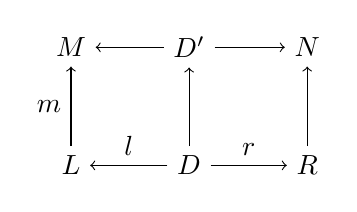
\begin{tikzpicture} %[scale=0.8]
    \node (l) at (-1.5,0) {\(L\)};
    \node (d) at (0,0) {\(D\)};
    \node (r) at (1.5,0) {\(R\)};
    \node (m) at (-1.5,1.5) {\(M\)};
    \node (d') at (0,1.5) {\(D'\)};
    \node (n) at (1.5,1.5) {\(N\)};
    \draw [->] (d) -- node [above,midway] {\(l\)} (l);
    \draw [->] (d) -- node [above,midway] {\(r\)} (r);
    \draw [->] (d') -- (m);
    \draw [->] (d') -- (n);
    \draw [->] (l) -- node [left,midway] {\(m\)}  (m);
    \draw [->] (d) -- (d');
    \draw [->] (r) -- (n);
  \end{tikzpicture}
  \]
  The inverse rule is defined as $p^{-} = R\overset{r}{\leftarrow} D \overset{l}{\rightarrow} L$.
\end{definition}

\begin{remark}
  The DPO approach only works, if we impose that the rules we consider do not have \emph{no side effects}, which is also called the \emph{the dangling points condition}: the nodes $x$ in $L$ such that $m(x)$ is the source or target of an edge $e$ in $M\setminus L$, are also nodes in $D$.

  Other graph rewriting techniques exists that allows such rules. However, we are interested in reversible rules, and the DPO approach gives us the inverse of a rule in a straightforward way. We plan to extend the current work to rules with side effect in the future.
\end{remark}

We denote $L\action R$ the span $L\overset{l}{\leftarrow} D \overset{r}{\rightarrow} R$.

\begin{definition}
  A transition system on graphs $TS = (Q,E,T,I,<,\dashv)$ is a transition system where :
  \begin{itemize}
  \item the states $Q$ are simples graphs;
  \item an event $e=(p:L\action R,m_k(G):L\to G)$ is a pair consisting of a rule $p:L\action R$ and a function $m_k$, that for a graph $G$, selects one matching $m_k :L\to G$. The label of an event is the rule $\labl(e) = p$.
  \item a transition $M\overset{p}{\action} N$ consists in a DPO rewriting step:
    \[
    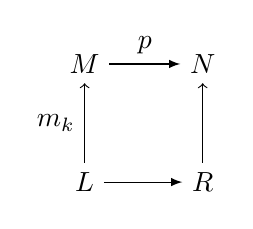
\begin{tikzpicture} %[scale=0.8]
      \node (l) at (-1.5,0) {\(L\)};
      \node (r) at (0,0) {\(R\)};
      \node (m) at (-1.5,1.5) {\(M\)};
      \node (n) at (0,1.5) {\(N\)};
      \draw [->] (l) -- node [left,midway] {\(m_k\)}  (m);
      \draw [>=latex, ->] (l) -- (r);
      \draw [>=latex, ->] (m) -- node [above,midway] {\(p\)} (n);
      \draw [->] (r) -- (n);
    \end{tikzpicture}
    \]
    where $p$ is the rule $L\action R$.
  \end{itemize}
\end{definition}



In the set of poset \mathcal{S}
